\documentclass[12pt,a4paper]{article}
\usepackage[utf8]{inputenc}
\usepackage[brazil]{babel}
\usepackage{graphicx}
\usepackage{amssymb, amsfonts, amsmath}
\usepackage{float}
\usepackage{enumerate}
\usepackage[top=1.5cm, bottom=1.5cm, left=1.25cm, right=1.25cm]{geometry}

\begin{document}
\pagestyle{empty}

\begin{center}
  \begin{tabular}{ccc}
    \begin{tabular}{c}
      
\includegraphics[scale=0.25]{../../biblioteca/imagem/brasao-de-armas-brasil} \\
    \end{tabular} & 
    \begin{tabular}{c}
      Ministério da Educação \\
      Universidade Federal dos Vales do Jequitinhonha e Mucuri \\
      Faculdade de Ciências Sociais, Aplicadas e Exatas - FACSAE \\
      Departamento de Ciências Exatas - DCEX \\
      Disciplina: Cálculo Diferencial e Integral I \quad Semestre: 2021/2\\
      Prof. Me. Luiz C. M. de Aquino\\
    \end{tabular} &
    \begin{tabular}{c}
      
\includegraphics[scale=0.25]{../../biblioteca/imagem/logo-ufvjm} \\
    \end{tabular}
  \end{tabular}
\end{center}

\begin{center}
  \textbf{Lista I}
\end{center}

\begin{enumerate}
  \item Analisando o gráfico da função $f$ ilustrado abaixo, responda aos quesitos.

  \begin{figure}[!tbh]
    \centering
    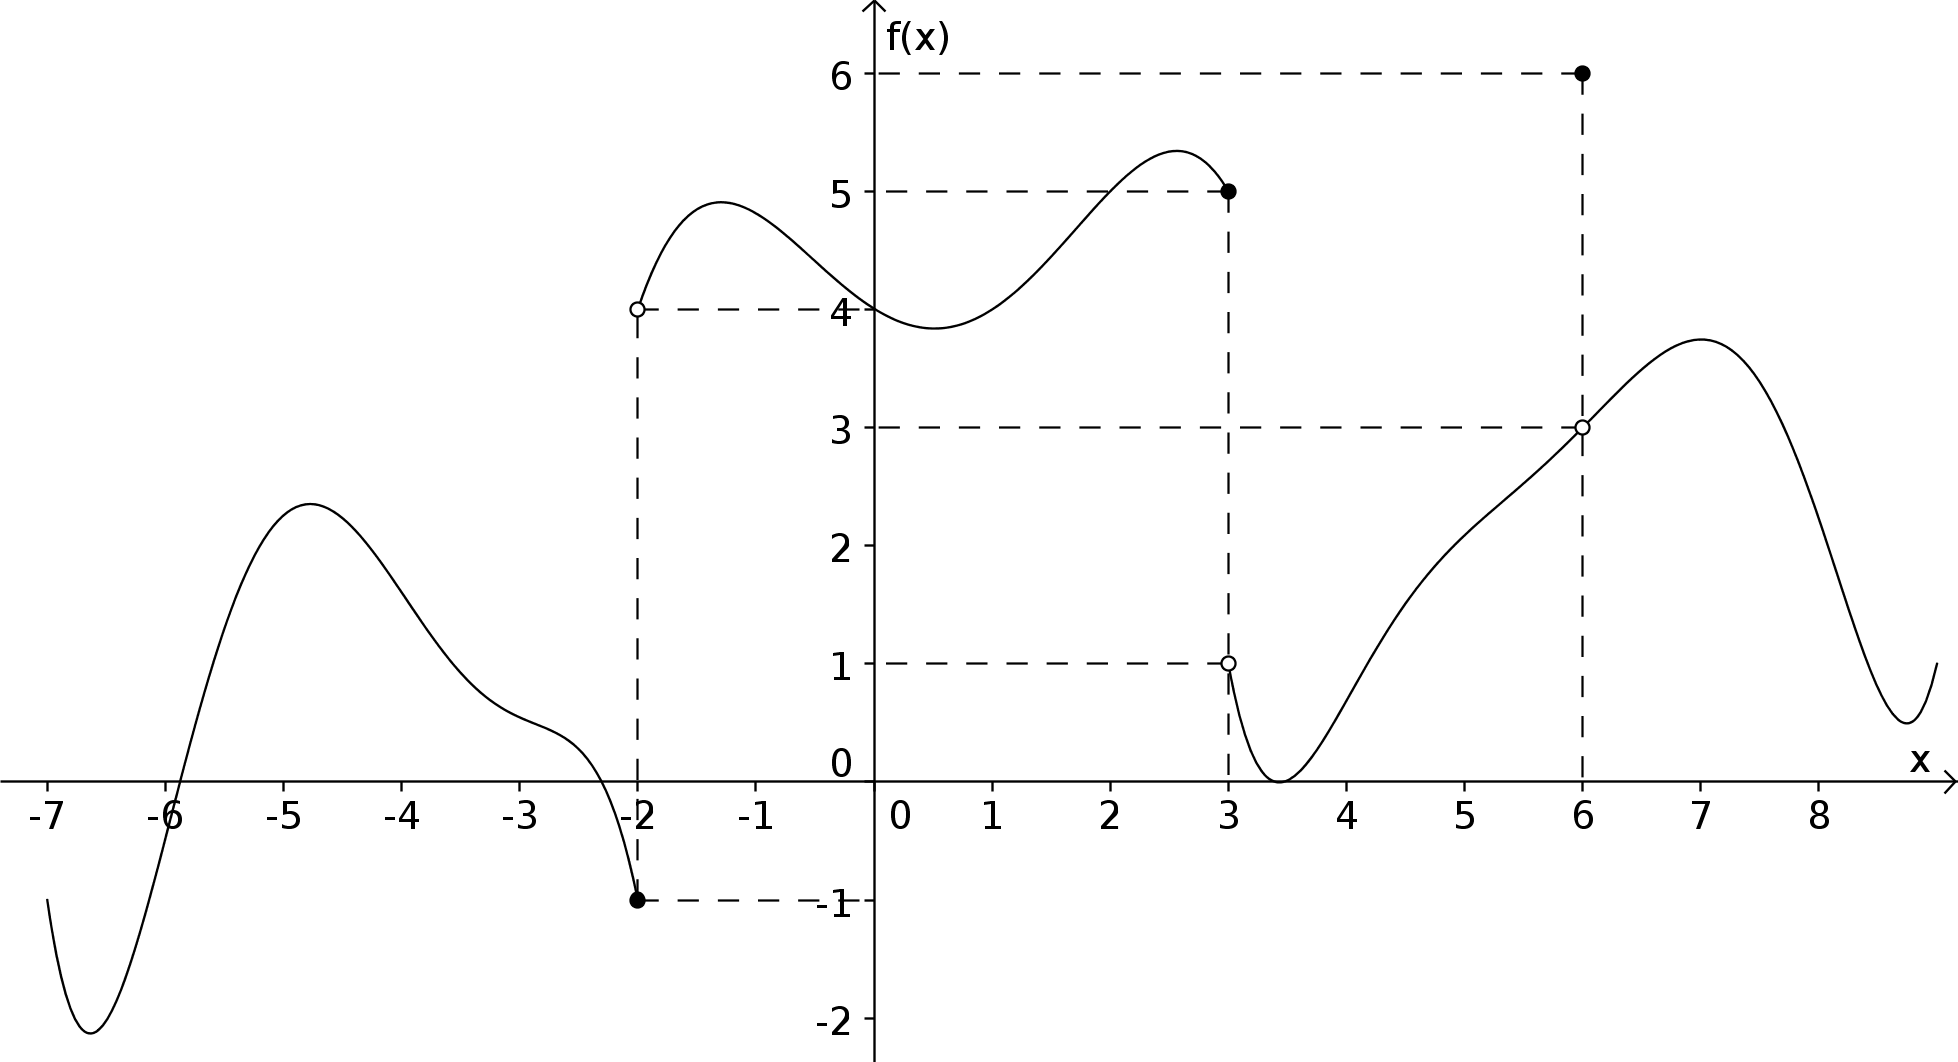
\includegraphics[scale=0.8]{imagem/grafico-lista2-questao1}
  \end{figure}

  \begin{tabular}{lll}
    (a) ${\displaystyle \lim_{x\to-2^{-}}f(x)}$ & (c) ${\displaystyle \lim_{x\to3^{-}}f(x)}$ & (e) ${\displaystyle \lim_{x\to6}f(x)}$ \\
    (b) ${\displaystyle \lim_{x\to-2^{+}}f(x)}$ & (d) ${\displaystyle \lim_{x\to3^{+}}f(x)}$ &
  \end{tabular}

  \item Considerando a função 
    $f(x)=\begin{cases}
      2x+16 & ;\, x<-3\\
      x^{2}-x-2 & ;\,-3\leq x<3\\
      \dfrac{10}{3}x-5 & ;\, x\geq3
    \end{cases}$, calcule os limites abaixo.

    \begin{tabular}{lll}
      (a) ${\displaystyle \lim_{x\to-3^{-}}f(x)}$ & (c) ${\displaystyle \lim_{x\to 1^{+}}f(x)}$ & (e) ${\displaystyle \lim_{x\to3^{-}}f(x)}$ \\
      (b) ${\displaystyle \lim_{x\to-3^{+}}f(x)}$ & (d) ${\displaystyle \lim_{x\to 1^{+}}f(x)}$ & (f) ${\displaystyle \lim_{x\to3^{+}}f(x)}$
    \end{tabular}

  \item Determine o valor da constante $c$ para que a função 
    $f(x)=\begin{cases}
      x^{2}-c^{2} & ;\, x < 4\\
      cx+20 & ;\, x \geq 4
    \end{cases}$ seja tal que ${\displaystyle \lim_{x\to4}f(x)=f(4)}$.

  \item Calcule o valor dos limites abaixo.
  
  \begin{tabular}{lll}
    (a) ${\displaystyle \lim_{x\to2}\dfrac{x^{2}-x-2}{x-2}}$ & (d)${\displaystyle \lim_{y\to9}\dfrac{9-y}{3-\sqrt{y}}}$ & (g) ${\displaystyle \lim_{x\to1}\dfrac{\sqrt{x}-x}{1-\sqrt{x}}}$ \\

    (b) ${\displaystyle \lim_{h\to0}\dfrac{(h-5)^{2}-25}{h}}$ & (e) ${\displaystyle \lim_{t\to7}\dfrac{\sqrt{t}-\sqrt{7}}{t-7}}$ &  (h) ${\displaystyle \lim_{m \to 1}\dfrac{m^3 - 1}{\sqrt{m} - 1}}$\\

    (c)${\displaystyle \lim_{t\to1}\dfrac{t^{2}+t-2}{t^{2}-3t+2}}$ & (f) ${\displaystyle \lim_{k\to 0}\dfrac{k}{\sqrt{2-k}-\sqrt{2}}}$ & \\
  \end{tabular}

  \item Em um estacionamento é cobrado R\$$2,00$ por cada intervalo de 30
    minutos (ou partes do mesmo). Com base nessa informação, responda
    aos quesitos abaixo.

    \begin{enumerate}
      \item Qual o valor pago por 20, 30 e 40 minutos?
      \item Seja $f$ a função que associa a quantidade de minutos de permanência
        no estacionamento com o valor pago pelo serviço. O limite ${\displaystyle \lim_{x\to15}f(x)}$
        existe? E quanto a ${\displaystyle \lim_{x\to30}f(x)}$? Justifique sua resposta.
      \item Esboce o gráfico da função $f$ do quesito anterior.
    \end{enumerate}

  \item Escolha um número positivo não nulo qualquer. Utilizando uma calculadora, calcule a sua raiz quadrada.
    Em seguida, calcule a raiz quadrada do resultado anterior. Continuando esse processo por várias vezes, o 
    resultado fica cada vez mais próximo de 1. Use os conceitos de limite para justificar esse fato.

  \item Na teoria da relatividade, a massa de uma partícula com velocidade $v$ é
  $$m = \dfrac{m_0}{\sqrt{1 - \dfrac{v^2}{c^2}}}$$
  onde $m_0$ é a massa da partícula em repouso e $c$ é a velocidade da luz. O
  que acontece quando $v\to c^-$?
  
  \item Prove que se $f$ é uma função contínua em $a$, então 
  $$\lim_{h\to 0} f(a + h) = f(a)$$
  
\end{enumerate}

\begin{center}
  \textbf{Gabarito}
\end{center}

\textbf{[1]} (a) -1. (b) 4. (c) 5. (d) 1. (e) 3. 
\textbf{[2]} (a) 10 (b) 10 (c) -2 (d) -2 (e) 4 (f) 5. 
\textbf{[3]} $c=-2$. 
\textbf{[4]} (a) 3. (b) -10. (c) -3. (d) 6. 
(e) $\frac{1}{2\sqrt{7}}$. (f) $-2\sqrt{2}$. 
(g) 1. (h) 6. 
\textbf{[5]} (a) 2, 2 e 4. (b) Sim. Não.
\textbf{[6]} Dica: note que $\displaystyle \lim_{n\to +\infty} x^\frac{1}{2^n} = 1$, onde $x\in\mathbb{R}_+^*$. 
\textbf{[7]} A massa $m$ tende ao infinito. 
\textbf{[8]} Dica: note que por definição de continuidade temos $\displaystyle \lim_{x\to a} f(x) = f(a)$. Aplique 
a substituição $x = a + h$. 
\end{document}